\documentclass[a4paper]{article}
\usepackage{geometry}
\usepackage{amsmath}
\usepackage{multicol}
\usepackage{graphicx}
\geometry{margin=0.25in}

\setlength{\parindent}{0pt}


\begin{document}
\begin{multicols}{3}
\raggedright
\fontsize{9pt}{0.3pt}\selectfont
\setlength{\abovedisplayskip}{2pt}
\setlength{\belowdisplayskip}{0pt}

% 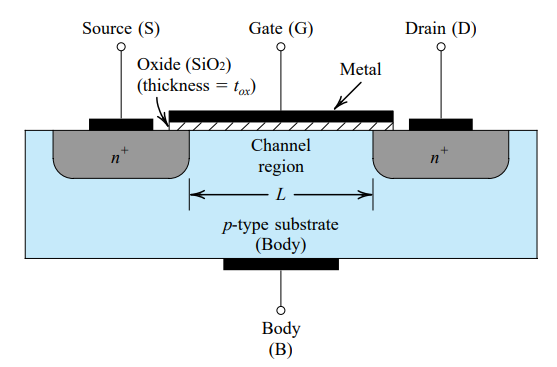
\includegraphics[width=\linewidth]{imgs/nmos}
The size of the "process" indicates the minimum
possible channel length. 

Magnitude of the electron charge in the channel [Q]:$$|Q|=C_{OX}(WL)v_{OV}$$
$C_{OX}$ is the oxide capacitance, [F/m$^2$]

$$C_{OX}=\frac{\epsilon_{OX}}{t_{OX}}$$

$\epsilon_{OX}$ is the permittivity of the SiO$_2$.\\
$t_{OX}$ is the oxide thickness.

For $C_{OX}$ per micron squared, use \\
$C=C_{OX}WL$ [fF]

$$i_D=\left[ (\mu_nC_{OX})\left(\frac{W}{L}\right)(v_{GS}-V_t)\right]v_{DS}$$
$$i_D=\left[ g_{DS} \right]v_{DS}$$
$$k_n^{'}=\mu_nC_{OX}$$
$$k_n=k_n^{'}(W/L)$$

$k_n^{'}$ is \textbf{process transconductance paramter}.\\
$k_n$ is \textbf{device transconductance paramter}.
\vspace{1mm}

When $V_{DS}$ is small, the MOSFET behaves as a linear 
resistance $r_{DS}$ whose value is controlled by the gate 
voltage $v_{GS}$.
$$r_{DS}=\frac{1}{g_{DS}}$$

% 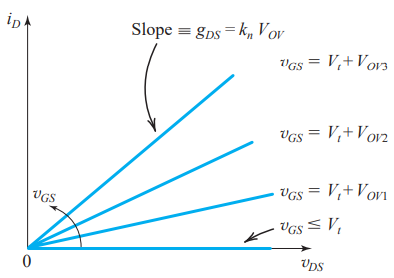
\includegraphics[width=\linewidth]{imgs/nmos_as_r}

\hrule
\vspace{1mm}
Triode vs Saturation

% 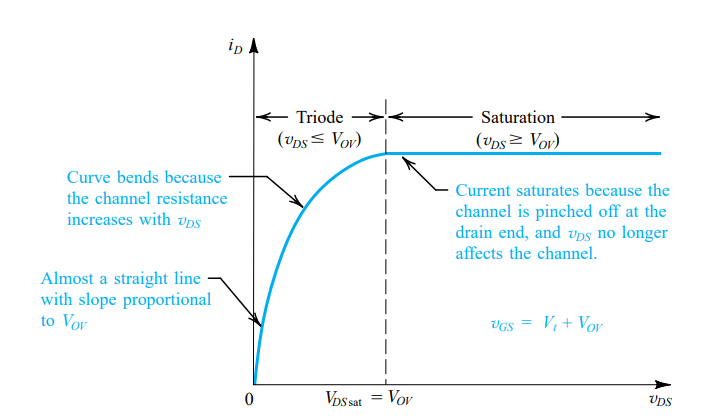
\includegraphics[width=\linewidth]{imgs/triode_sat.png}

Triode ($v_{DS} \leq V_{OV}$)

$$i_D=k_n^{'}\left(\frac{W}{L}\right)\left(V_{OV}-\frac{1}{2}v_{DS}\right)v_{DS}$$
$$i_D=k_n^{'}\left(\frac{W}{L}\right)\left[(v_{GS}-V_t)v_{DS}-\frac{1}{2}v_{DS}^2\right]$$

Saturation ($v_{DS} \geq V_{OV}$)

$$i_D=\frac{1}{2}k_n^{'}\left(\frac{W}{L}\right)V_{OV}^2$$
$k_n=k_n^{'}$, so
$$i_D=\frac{1}{2}k_nV_{OV}^2$$
Or,
$$i_D=\frac{1}{2}k_n(V_{GS}-V_{th})^2$$

% 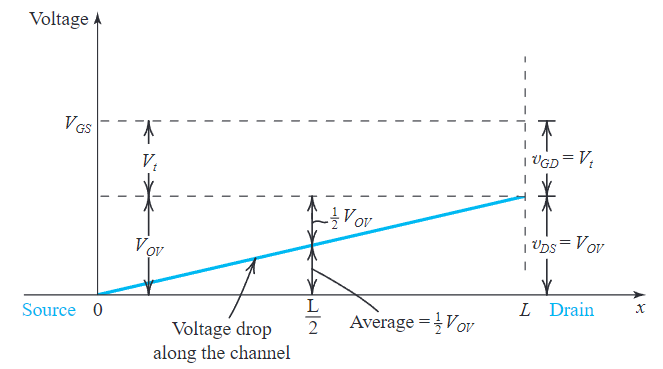
\includegraphics[width=\linewidth]{imgs/mosfet_sat.png}

Constant $V_{OV}$ can be replaced by variable $v_{OV}$.

PMOS transistors operate similarly but the polarity is
reversed, so $v_{GS}$ must be negative and larger than 
a negative $v_{tp}$, as is $v_{DS}$ negative.

% 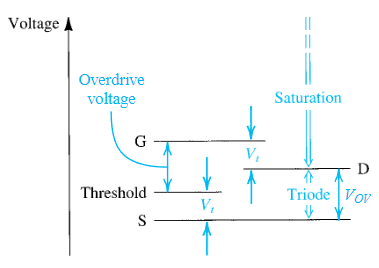
\includegraphics[width=\linewidth]{imgs/mosfet_operation.png}

If you care about \textbf{channel-length modulation}, then use
the expression:
$$i_D=\frac{1}{2}k_n^{'}\left(\frac{W}{L}\right)(v_{GS}-V_{th})^2(1+\lambda v_{DS})$$

$v_{DS}=-\frac{1}{\lambda} \mid$
$V_A=\frac{1}{\lambda} \mid$
$V_A=V_A^{'}L$  

$V_A$ (Early Voltage) has units of volts.\\
$V_A^{'}$ has units of volts per micron.

% 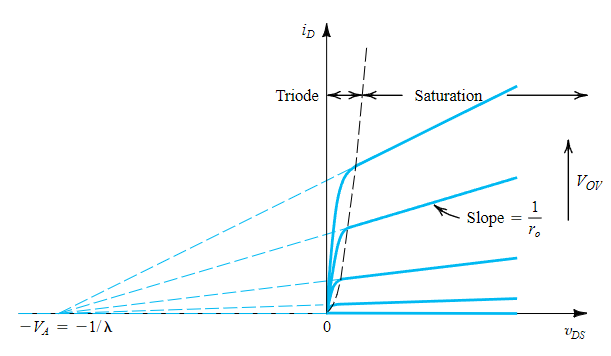
\includegraphics[width=\linewidth]{imgs/va_mosfet.png}

Expression for $r_o$:
$$r_o=\frac{V_A}{I_D}=\frac{1}{\lambda I_D}$$
$I_D$ is the drain current without channel-length
modulation taken into account.
$$I_D=\frac{1}{2}k_n^{'}\frac{W}{L}(V_{GS}-V_{tn})^2$$

For a $p$-Channel MOSFET, everything is backwards, here is an
equation showing the voltages without negative signs, everything
here is considered in terms of positive voltages or magnitudes.
$$i_D=\frac{1}{2}k_p^{'}\left(\frac{W}{L}\right)(v_{SG}-|V_{tp}|)^2(1+|\lambda|v_{SD})$$
Also,
$$i_D=\frac{1}{2}k_p^{'}\left(\frac{W}{L}\right)(v_{SG}-|V_{tp}|)^2\left(1+\frac{v_{SD}}{|V_A|}\right)$$
Kinda useful:
$$R_D=\frac{V_{DD}-V_D}{I_D}$$
$$R_D=V_{DD}-I_D R_D$$
% 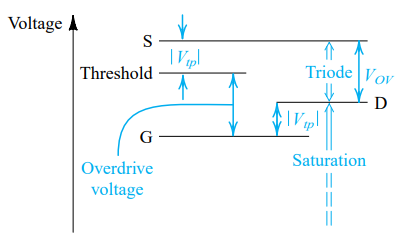
\includegraphics[width=\linewidth]{imgs/pmos_operation.png}

\hrule
\vspace{1mm}
MOSFETs biased for linear amplification
% 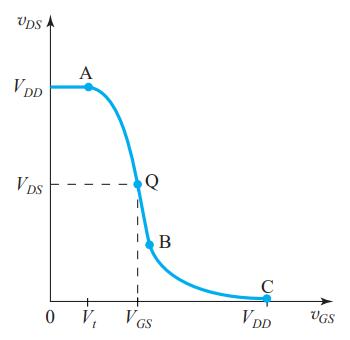
\includegraphics[width=\linewidth]{imgs/bias_point_q.png}
Note \textbf{bias point Q}.
Voltages $V_{GS}$ and $V_{DS}$ are related at the bias point
by 
$$v_{DS}=V_{DD}-\frac{1}{2}k_n R_D (v_{GS}-V_t)^2$$
$$v_{GS}=V_{GS}+v_{gs}$$

% 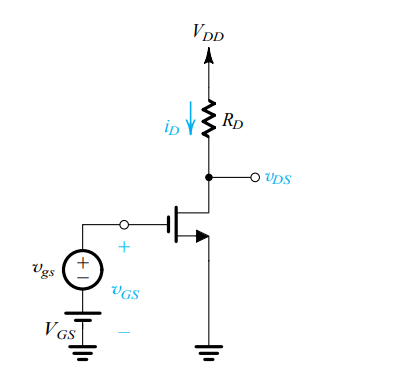
\includegraphics[width=\linewidth]{imgs/nmos_as_amp1.png}

$A_v$ is expressed in terms of $V_{OV}$ at the bias point by
$$A_v=-k_n V_{OV} R_D$$
$$A_v=-\frac{2 I_D R_D}{V_{OV}}=-\frac{I_D R_D}{V_{OV}/2}$$

To prevent \emph{nonlinear distortion}, $v_{gs}$ must be sufficiently
small.
$$v_{gs} \ll 2(V_{GS} - V{t})$$
$$v_{gs} \ll 2V_{OV}$$

When this condition is met, we can express $i_D$ as:
$$i_D \simeq I_D + i_d$$
Of course, $I_D=\frac{1}{2}k_n V_{OV}^2$\\
and $i_d=k_n(V_{GS}-V_t)v_{gs}$

$$g_m \equiv \frac{i_d}{v_{gs}} = k_n(V_{GS}-V_t)$$
$$g_m = k_n V_{OV}=\mu_n C_{ox} \frac{W}{L} V_{OV}$$
$$g_m = k_n^{'}(W/L)(V_{GS}-V_t)=k_n^{'}(W/L)V_{OV}$$
$$g_m = \sqrt{2k_n^{'}}\sqrt{W/L}\sqrt{I_D}$$
$$g_m = \frac{2I_D}{V_{GS}-V_t}=\frac{2I_D}{V_{OV}}=\sqrt{2\mu_n C_{ox} \frac{W}{L} I_D}$$

\hrule
\vspace{1mm}
Small Signal Model
% 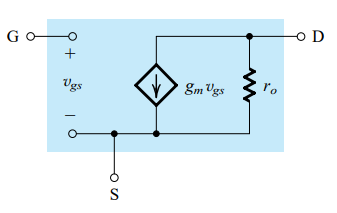
\includegraphics[width=\linewidth]{imgs/small_signal_model}
$r_o=\frac{|V_A|}{I_D}=\frac{1}{\lambda I_D} \mid A_v=\frac{v_{ds}}{v_{gs}}=-g_m(R_D\parallel r_o)$

$$v_{DS} = V_{DD} - R_D i_D$$
$$v_{DS} = V_{DD} - R_D(I_D + i_d) = V_{DS} - R_D i_d$$

$$v_{DS} = -i_d R_D = -g_m v_{gs} R_D$$
$$A_v \equiv \frac{v_{ds}}{v_{gs}} = -g_m R_D$$

\hrule
\vspace{1mm}
T Equivalent-Circuit Model
% 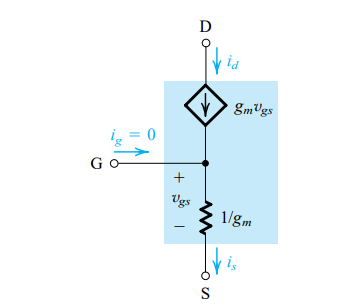
\includegraphics[width=\linewidth]{imgs/t_circuit.png}

$i_d=i_s=g_m v_{gs}$
\end{multicols}
\pagebreak
\begin{multicols*}{3}
\columnbreak

\hrule
\vspace{1mm}
Characterizing Amplifiers

% 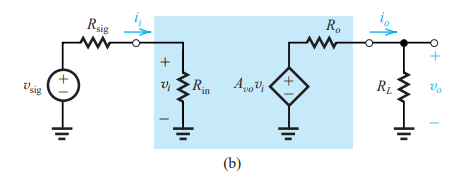
\includegraphics[width=\linewidth]{imgs/amplifier_model.png}
$$A_{vo} \equiv \frac{v_o}{v_i} \Big|_{R_L=\infty}$$
$$A_v \equiv \frac{v_o}{v_i} = A_{vo} \frac{R_L}{R_L + R_o}$$
$$G_v \equiv \frac{v_o}{v_\text{sig}}$$
    
\hrule
\vspace{1mm}
Basic circuit configurations

% 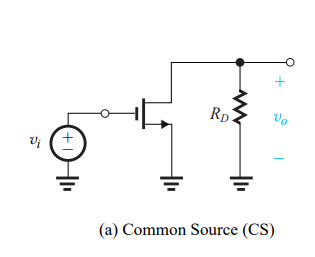
\includegraphics[width=0.8\linewidth]{imgs/common_source.png}

$R_{\text{in}}=\infty \mid v_o=-(g_mv_{gs})(R_D \parallel r_o)$\\
$A_{vo}=-g_m(R_D \parallel r_o)$\\
$A_v = G_v =-g_m(R_D \parallel R_L \parallel r_o)$

$v_{\text{sig}}$ must be much smaller than $2V_{OV}$

% 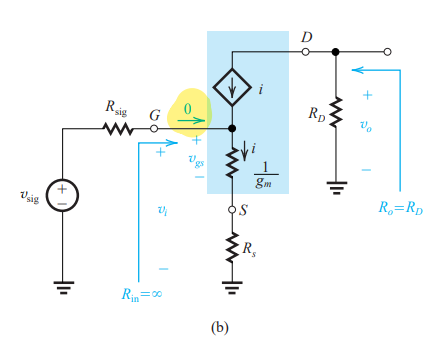
\includegraphics[width=\linewidth]{imgs/cs_rs.png}
$$v_{gs}=\frac{v_i}{1+g_mR_s}$$
$$v_o=-i R_D$$
$$i = \frac{v_i}{1/g_m + R_s} = \left(\frac{g_m}{1+g_m R_s}\right)v_i$$
Those two together make:
$$A_{vo}=\frac{v_o}{v_i} = -\frac{R_D}{1/g_m + R_s}$$
$$A_v=-\frac{R_D \parallel R_L}{1/g_m + R_s}$$

\hrule
% 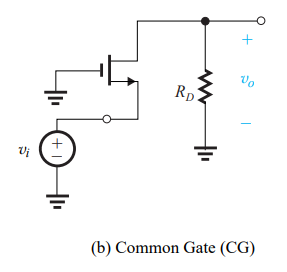
\includegraphics[width=0.8\linewidth]{imgs/common_gate.png}

$R_\text{in}=\frac{1}{g_m} \mid i=-\frac{v_i}{1/g_m} \mid v_o=-i R_D$\\
$$A_{vo} \equiv \frac{v_o}{v_i} = g_m R_D$$

$$G_v= \frac{(R_D \parallel R_L)}{R_\text{sig}+1/ g_m}$$

\hrule
% 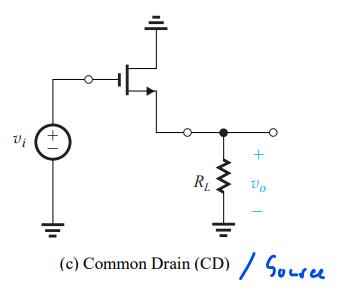
\includegraphics[width=0.8\linewidth]{imgs/common_drain.png}

Often used as a voltage buffer so that the signal isn't attenuated
at the output.

$R_\text{in}=\infty \mid A_{vo}=1 \mid R_o=1/g_m$
$$G_v=A_v=\frac{R_L}{R_L+1/g_m}$$

\hrule
\vspace{1mm}
Biasing amplifier circuits

Fixing $V_G$ and using $R_s$, use\\
$V_G=V_{GS}+R_sI_D$

\vspace{1cm}
Depletion-type MOSFET is the same as normal mosfet but 
it has a negative $V_t$ (positive for PMOS).
\end{multicols*}

\end{document}
